\documentclass[UTF8,a4paper,12pt,oneside]{ctexrep}

\usepackage{geometry}
\usepackage{setspace}
\usepackage{graphicx}
\usepackage{booktabs}
\usepackage{longtable}
\usepackage{tabularx}
\usepackage{array}
\usepackage{enumitem}
\usepackage{xcolor}
\usepackage{listings}
\usepackage{hyperref}
\usepackage{fancyhdr}
\usepackage{titlesec}
\usepackage{caption}
\usepackage{float}
\usepackage{tikz}
\usetikzlibrary{arrows.meta,positioning,fit,shapes.geometric}

\geometry{left=2.8cm,right=2.8cm,top=2.8cm,bottom=2.8cm}
\onehalfspacing
\setlength{\parindent}{2em}
\setlength{\parskip}{0.25em}
\setlist[itemize]{leftmargin=2.5em}
\setlist[enumerate]{leftmargin=2.7em}

\hypersetup{
  colorlinks=true,
  linkcolor=black,
  urlcolor=blue,
  citecolor=black,
  pdfauthor={seccomp-privacy-platform team},
  pdftitle={面向电商场景的隐私计算平台设计与实现}
}

\pagestyle{fancy}
\setlength{\headheight}{15pt}
\fancyhf{}
\fancyhead[C]{面向电商场景的隐私计算平台设计与实现}
\fancyfoot[C]{\thepage}
\renewcommand{\headrulewidth}{0.4pt}

\ctexset{
  chapter = {
    name = {第,章},
    number = \chinese{chapter},
    format = \centering\zihao{3}\heiti,
    beforeskip = 12pt,
    afterskip = 18pt
  },
  section = {
    format = \zihao{4}\heiti,
    beforeskip = 12pt,
    afterskip = 6pt
  },
  subsection = {
    format = \zihao{-4}\heiti,
    beforeskip = 8pt,
    afterskip = 4pt
  }
}

\lstdefinestyle{codestyle}{
  basicstyle=\ttfamily\small,
  breaklines=true,
  frame=single,
  columns=fullflexible,
  keepspaces=true,
  backgroundcolor=\color{gray!5},
  rulecolor=\color{gray!50},
  keywordstyle=\color{blue!70!black},
  commentstyle=\color{green!40!black},
  stringstyle=\color{red!60!black}
}
\lstset{style=codestyle}

\newcommand{\project}{seccomp-privacy-platform}
\newcommand{\pipeline}{SSE candidate export $\rightarrow$ controlled record recovery $\rightarrow$ Rust bridge tokenization $\rightarrow$ A-PSI/PJC $\rightarrow$ policy release}
\newcommand{\filepath}[1]{\texttt{\detokenize{#1}}}

\begin{document}

\begin{titlepage}
  \centering
  \vspace*{1.5cm}
  {\zihao{2}\heiti 面向电商场景的隐私计算平台\\[0.3em]设计与实现\par}
  \vspace{1.2cm}
  {\zihao{3}\bfseries 项目报告\par}
  \vspace{2.2cm}
  \begin{tabular}{>{\bfseries}r l}
    作品名称： & 面向电商场景的隐私计算平台 \\
    项目仓库： & \project \\
    技术方向： & 可搜索加密、受控数据恢复、隐私集合计算、审计治理 \\
    适用场景： & 电商与广告平台跨方归因、隐私查询与聚合发布 \\
    报告版本： & 结题报告草案 \\
    日期： & \today \\
  \end{tabular}
  \vfill
  {\zihao{-4}本报告依据项目代码、README、docs、schemas、handoff 与 report 目录参考文档整理。\par}
\end{titlepage}

\pagenumbering{Roman}

\chapter*{摘要}
\addcontentsline{toc}{chapter}{摘要}

在电商、广告投放、风控和合规审计等场景中，不同机构之间往往需要进行跨方用户匹配与聚合分析。例如，广告平台希望评估投放转化效果，电商平台希望在不泄露订单明细和用户标识的前提下完成归因统计。传统明文数据交换会暴露电子邮箱、手机号、设备标识、订单金额、活动标签等敏感信息；仅依赖普通访问控制又难以证明中间过程没有越权恢复、重复查询或结果泄露。因此，构建一条具备候选检索、受控恢复、匿名化联结、安全计算、策略发布和审计追溯能力的隐私计算链路具有现实意义。

本项目实现了一个面向电商隐私数据场景的比赛版平台基线，主链路为：\pipeline。系统由 \filepath{sse/}、\filepath{services/record_recovery/}、\filepath{bridge/}、\filepath{a-psi/}、\filepath{scripts/}、\filepath{schemas/} 等模块组成。其中，SSE 模块负责密文可搜索存储与候选导出；record recovery 服务负责在策略约束下恢复最小必要字段；Rust bridge 模块负责 join key 规范化、HMAC token 生成和 PJC 输入准备；A-PSI/PJC 模块负责隐私集合交集与聚合求和；policy release 模块负责阈值发布、防重复查询和公开报告生成。围绕主链路，项目还实现了 metadata sidecar、query workflow、operator dashboard、audit chain、schema contract、benchmark、health check、malformed input gate 与 audit tamper resistance 等平台化能力。

当前代码已经超过单纯原型演示，能够在本地和 live SSE demo 中完成端到端验证，标准示例结果为 \texttt{intersection\_size=2}、\texttt{intersection\_sum=425}。同时，项目明确保留阶段边界：它是平台基线和比赛版隐私计算系统，不应被描述为完整生产级多租户电商平台、完整 customer 360 数据底座或长期托管的真实 Keycloak/OpenFGA/Vault/AWS KMS 生产环境。

\noindent\textbf{关键词：} 可搜索加密；隐私集合计算；Private Join and Compute；数据恢复服务；电商隐私平台；审计链；策略发布

\tableofcontents
\clearpage
\pagenumbering{arabic}

\chapter{作品概述}

\section{研究背景}

电商平台和广告平台之间的跨方归因是隐私计算的典型场景。广告平台掌握曝光或点击侧用户标识，电商平台掌握订单、支付、履约和客服等业务事实。双方希望得到交集用户数量、成交金额等聚合指标，却不能直接交换原始用户标识或订单明细。如果将电子邮箱、手机号、设备 ID、订单金额等字段以明文方式传递给对方或第三方计算服务，会带来以下风险：

\begin{enumerate}
  \item 原始 join key 泄露，导致跨库用户画像拼接。
  \item 候选集合过细，导致对某些用户是否参与活动进行推断。
  \item 查询被重复或微调执行，产生差分攻击和重识别风险。
  \item 中间产物缺少审计链，事后无法证明哪些字段被恢复、哪些结果被发布。
  \item 运维人员或服务调用方越权读取临时明文 handoff 文件。
\end{enumerate}

因此，本项目的目标不是构建一个普通数据仓库，而是在隐私计算主链路上实现“最小恢复、最小暴露、可验证审计、受控发布”的平台基线。

\section{项目目标}

项目目标可概括为四点：

\begin{enumerate}
  \item 建立一条可复现的端到端隐私计算链路，完成候选检索、受控恢复、token 化、PJC 计算和策略发布。
  \item 对跨模块接口进行 contract 固化，避免多人协作时静默改变 \texttt{caller}、\texttt{tenant\_id}、\texttt{dataset\_id}、\texttt{service\_id}、\texttt{job\_id}、\texttt{correlation\_id} 等核心语义。
  \item 建立审计、观测、benchmark 和平台健康检查等 sidecar 能力，使运行结果可解释、可回放、可取证。
  \item 面向电商场景补齐权限画像、事实层基线和团队交付材料，使项目能够用于 pre 汇报和结题报告。
\end{enumerate}

\section{工作内容}

项目工作可以分为六条线：

\begin{enumerate}
  \item \textbf{隐私计算主链路。} 实现 \pipeline 的完整流程，示例输出为交集数量 2、交集金额 425。
  \item \textbf{恢复服务边界。} 将 encrypted record store 的候选行恢复逻辑从 \filepath{sse/toolkit/} 迁移到 \filepath{services/record_recovery/}，支持 Unix socket、HTTP、mTLS、health、audit、authz 和 runtime log。
  \item \textbf{Rust bridge。} 实现 join key normalization、HMAC-SHA256 token、\texttt{server.csv}/\texttt{client.csv}/\texttt{job\_meta.json} 生成，以及 bridge audit。
  \item \textbf{策略与审计治理。} 实现 export policy、release policy、duplicate-query deny、audit chain、seal、archive、tamper resistance。
  \item \textbf{平台 sidecar。} 实现 metadata DB、query workflow、operator dashboard、platform health、observability、catalog lineage、benchmark。
  \item \textbf{电商平台叙事。} 落地 Track-E1 电商事实层 6 表基线、Track-E2 业务身份注解、Track-E3 operator console/request workflow 基线。
\end{enumerate}

\section{应用前景}

本项目可用于以下场景：

\begin{itemize}
  \item 广告平台与电商平台之间进行隐私保护归因，输出交集人数和交易金额。
  \item 营销活动复盘，按 campaign 或渠道统计被允许发布的聚合结果。
  \item 风控场景中对疑似风险集合与订单集合做隐私保护交集分析。
  \item 合规审计场景中复核隐私查询的 caller、scope、policy、audit chain 是否一致。
  \item 教学和比赛展示中演示 SSE、record recovery、HMAC tokenization、PJC 和审计治理的组合式平台设计。
\end{itemize}

\chapter{背景知识与预备概念}

\section{可搜索对称加密}

可搜索对称加密（Searchable Symmetric Encryption, SSE）允许数据持有方在加密数据上建立可搜索索引，使服务器能够在不知道明文内容的情况下返回候选记录标识。本项目中的 \filepath{sse/} 基于 SSEPy 原型扩展，承担两个角色：

\begin{enumerate}
  \item 维护可搜索加密存储和检索服务。
  \item 在 export policy 约束下，将 SSE 搜索结果转化为 bridge-ready 候选导出。
\end{enumerate}

在隐私边界上，SSE 阶段允许泄露候选数量、角色、调用者、过滤条件 hash 和输出 hash，不允许将原始过滤值、原始 join key 或 token secret 写入审计。

\section{受控记录恢复}

SSE 搜索得到的是候选 ID，而 PJC 需要的是规范化后的 join key 和必要 value 字段。record recovery 的作用是从 encrypted record store 中恢复被策略允许的候选行，并将恢复结果写入 bridge handoff。项目中的 encrypted record store 使用 PBKDF2HMAC-SHA256、AES-256-GCM 和 keyed HMAC-SHA256 record-id tag，避免直接暴露原始 record ID。

恢复服务边界实现位于 \filepath{services/record_recovery/}，旧的 \filepath{sse/toolkit/record_recovery_*.py} 文件只保留兼容 shim。该设计减少了 SSE CLI 与恢复业务逻辑的耦合，也让恢复服务可以作为独立 deploy unit 进行 health check、authz、structured log 和 mTLS 测试。

\section{Private Join and Compute}

Private Join and Compute（PJC）用于在双方不直接暴露原始集合成员的情况下计算交集及交集上 value 的聚合。本项目采用 \filepath{a-psi/} 中的 Private Join and Compute 工作流：server 通常代表广告或曝光侧，client 通常代表电商转化侧。bridge 将双方原始 join key 规范化并 HMAC token 化后，生成 PJC 所需的 \texttt{server.csv} 和 \texttt{client.csv}。

当前 demo 中，最终发布结果为：

\begin{lstlisting}[language=bash]
intersection_size=2
intersection_sum=425
\end{lstlisting}

\section{策略发布与审计}

PJC 的原始结果不能直接对外发布，需要经过 policy release。release 阶段负责：

\begin{enumerate}
  \item 阈值检查，例如 \texttt{k} 和 \texttt{n}。
  \item duplicate-query deny，拒绝对同一 caller 的完全重复查询。
  \item 生成 \texttt{public\_report.json} 和 release audit。
  \item 将 PJC result hash、decision、reason code 与 \texttt{correlation\_id} 写入审计链。
\end{enumerate}

\chapter{需求分析}

\section{功能需求}

\begin{longtable}{p{0.22\textwidth}p{0.68\textwidth}}
\toprule
\textbf{需求} & \textbf{说明} \\
\midrule
候选检索 & 支持通过 SSE keyword 和过滤条件选择候选记录。 \\
受控导出 & export policy 必须约束 caller、role、join key、value field、filter 和 row count。 \\
记录恢复 & 从 encrypted record store 中恢复最小必要字段，支持 subprocess、Unix socket 和 HTTP service。 \\
桥接处理 & 对 join key 进行 normalization 和 scoped HMAC tokenization，生成 PJC 输入。 \\
PJC 执行 & 计算双方 token 集合交集数量和 client value 聚合。 \\
策略发布 & 根据阈值、重复查询和 release policy 判断是否发布结果。 \\
审计链 & 记录 SSE export、record recovery、bridge、PJC、policy release 等阶段审计。 \\
可观测 & 输出 platform health、pipeline observability、catalog lineage 和 benchmark 报告。 \\
\bottomrule
\end{longtable}

\section{安全需求}

安全需求包括：

\begin{enumerate}
  \item 原始 join key 不进入 PJC，不写入 audit。
  \item record-store passphrase 和 bridge token secret 不出现在命令输出和审计中。
  \item recovery service 必须绑定 \texttt{caller}/\texttt{tenant\_id}/\texttt{dataset\_id}/\texttt{service\_id}。
  \item file handoff 的明文暴露必须可审计，优先支持 FIFO handoff。
  \item 审计文件必须可 seal、archive、verify，并可检测篡改。
  \item malformed input、错误 token、过期 timestamp、越权 scope 等请求必须被拒绝。
\end{enumerate}

\section{非功能需求}

\begin{itemize}
  \item \textbf{可复现性：} 提供 \texttt{run\_live\_sse\_bridge\_demo.sh}、\texttt{check\_json\_contracts.sh}、\texttt{check\_ci\_smoke.sh} 等固定入口。
  \item \textbf{可维护性：} 通过 \filepath{schemas/} 固化 JSON contract，通过 \texttt{check\_schema\_backcompat.py} 防止破坏性字段漂移。
  \item \textbf{可扩展性：} 外部 Keycloak、OpenFGA、Vault、AWS KMS、PostgreSQL、Grafana/Tempo 等均以 adapter 或 repo-side topology 方式接入，不强制改变主链路。
  \item \textbf{协作性：} 三人分工文档位于 \filepath{docs/team/TEAM_COLLABORATION_AND_REPORTING_PLAN.md}，明确 Person 1/2/3 的环境、任务和证据交付。
\end{itemize}

\chapter{系统总体设计}

\section{总体架构}

系统总体架构如图 \ref{fig:pipeline} 所示。

\begin{figure}[H]
\centering
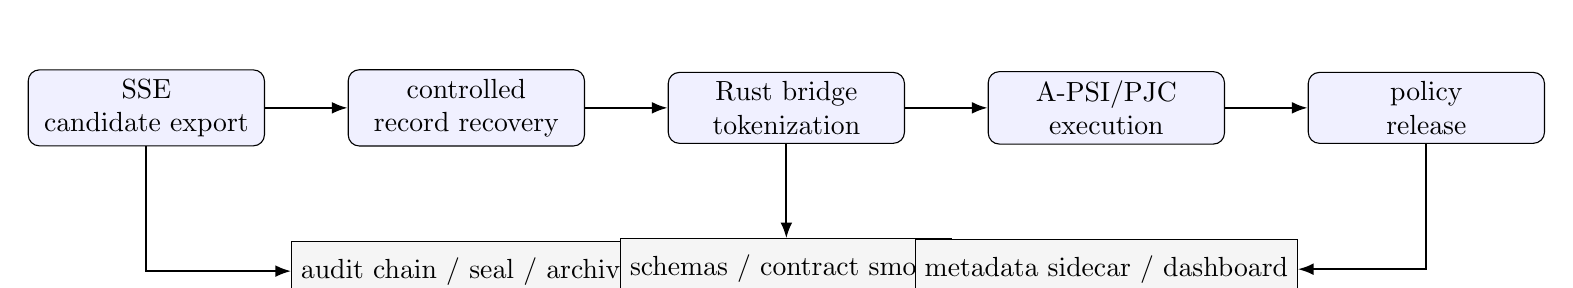
\begin{tikzpicture}[
  node distance=1.05cm,
  stage/.style={rectangle,rounded corners,draw=black,fill=blue!6,minimum width=3.0cm,minimum height=0.9cm,align=center},
  side/.style={rectangle,draw=black,fill=gray!8,minimum width=3.2cm,minimum height=0.75cm,align=center},
  arrow/.style={-{Latex[length=2mm]},thick}
]
  \node[stage] (sse) {SSE\\candidate export};
  \node[stage,right=of sse] (rec) {controlled\\record recovery};
  \node[stage,right=of rec] (bridge) {Rust bridge\\tokenization};
  \node[stage,right=of bridge] (pjc) {A-PSI/PJC\\execution};
  \node[stage,right=of pjc] (release) {policy\\release};

  \draw[arrow] (sse) -- (rec);
  \draw[arrow] (rec) -- (bridge);
  \draw[arrow] (bridge) -- (pjc);
  \draw[arrow] (pjc) -- (release);

  \node[side,below=1.2cm of rec] (audit) {audit chain / seal / archive};
  \node[side,below=1.2cm of bridge] (schema) {schemas / contract smoke};
  \node[side,below=1.2cm of pjc] (meta) {metadata sidecar / dashboard};

  \draw[arrow] (sse.south) |- (audit.west);
  \draw[arrow] (bridge.south) -- (schema.north);
  \draw[arrow] (release.south) |- (meta.east);
\end{tikzpicture}
\caption{隐私计算平台主链路与 sidecar 能力}
\label{fig:pipeline}
\end{figure}

\section{模块划分}

\begin{longtable}{p{0.24\textwidth}p{0.66\textwidth}}
\toprule
\textbf{目录或模块} & \textbf{职责} \\
\midrule
\filepath{sse/} & SSE 原型、客户端 CLI、搜索、受控 bridge export、policy gate。 \\
\filepath{services/record_recovery/} & encrypted record store、candidate row recovery、Unix socket/HTTP 服务、authz、health、runtime log。 \\
\filepath{bridge/} & Rust bridge，负责 normalization、HMAC tokenization、PJC input、job metadata、bridge audit。 \\
\filepath{a-psi/} & PJC 执行、bridge job validation、policy release、public report、policy audit。 \\
\filepath{scripts/} & 主链路编排、key agent、external KMS、metadata sidecar、operator dashboard、benchmark、audit 工具。 \\
\filepath{schemas/} & versioned JSON schema contracts，覆盖 policy、audit、metadata、benchmark、health、workflow 等。 \\
\filepath{migrations/metadata/} & SQLite metadata sidecar migrations，包含控制面、key registry、OpenFGA tuples、service tokens、电商事实层和 workflow submissions。 \\
\filepath{docs/} & 架构、路线图、威胁模型、runbook、benchmark、合规映射和团队协作文档。 \\
\bottomrule
\end{longtable}

\section{核心数据流}

一次典型查询的数据流如下：

\begin{enumerate}
  \item 查询请求指定 server/client source、join key 字段、value 字段、filter、caller、tenant、dataset、service、token scope 和 release 参数。
  \item SSE export 根据 policy 校验 caller 权限，并根据 keyword/filter 生成候选集合。
  \item record recovery 根据候选 ID 从 encrypted record store 中恢复必要字段，生成 bridge-ready row。
  \item bridge 对 email 等 join key 进行 normalization，并使用 \texttt{token\_scope} 和 token secret 生成 HMAC token。
  \item PJC 使用 tokenized \texttt{server.csv} 和 \texttt{client.csv} 计算交集数量与金额聚合。
  \item policy release 根据阈值、重复查询和发布策略决定是否生成 public report。
  \item audit chain 将各阶段审计串联，供 mainline contract check、archive、verify 和 observability 使用。
\end{enumerate}

\section{冻结字段与接口治理}

多人协作时最容易产生隐私边界漂移，因此项目冻结以下字段语义：

\begin{center}
\begin{tabularx}{0.95\textwidth}{lX}
\toprule
\textbf{字段} & \textbf{含义} \\
\midrule
\texttt{job\_id} & 一次隐私查询或 pipeline run 的任务标识。 \\
\texttt{correlation\_id} & 跨 SSE、recovery、bridge、PJC、release 的审计关联标识。 \\
\texttt{caller} & 发起查询或操作的调用主体。 \\
\texttt{tenant\_id} & 租户 scope。 \\
\texttt{dataset\_id} & 数据集 scope。 \\
\texttt{service\_id} & 恢复服务或数据服务 scope。 \\
\texttt{record\_recovery\_boundary} & 表示恢复发生在 subprocess、service socket 或 service HTTP 边界。 \\
\texttt{token\_scope} & HMAC token 的作用域，必须在同一 PJC job 中一致。 \\
\texttt{token\_key\_version} & 参与 token 生成的密钥版本。 \\
\texttt{release\_policy} & 结果发布时使用的策略。 \\
\bottomrule
\end{tabularx}
\end{center}

\chapter{作品实现}

\section{SSE 导出与策略门禁}

SSE controlled export 的入口是：

\begin{lstlisting}[language=bash]
cd sse
.venv/bin/python run_client.py export-bridge-records \
  --source-path examples/bridge_client_records.jsonl \
  --out-path exports/client_demo.csv \
  --role client \
  --source-format jsonl \
  --out-format csv \
  --join-key-field email \
  --value-field amount \
  --filter campaign=demo \
  --caller auto_demo \
  --policy-config config/export_policy.example.json \
  --audit-log exports/export_audit.jsonl \
  --job-id auto_demo_job
\end{lstlisting}

该命令默认要求 policy config。若无策略，必须显式传入 unsafe flag，这降低了误用风险。审计日志记录 row count、filter hash、output hash、candidate source 和 decision，不记录原始 join key。

\section{Encrypted Record Store 与恢复服务}

encrypted record store 的创建示例：

\begin{lstlisting}[language=bash]
export SSE_RECORD_STORE_PASSPHRASE=<passphrase>
cd sse
.venv/bin/python run_client.py create-encrypted-record-store \
  --source-path examples/bridge_client_records.jsonl \
  --out-path exports/client_records.enc.jsonl \
  --source-format jsonl \
  --record-id-field email_hex \
  --key-env SSE_RECORD_STORE_PASSPHRASE
\end{lstlisting}

恢复服务推荐入口：

\begin{lstlisting}[language=bash]
python3 scripts/run_record_recovery_service.py serve \
  --config config/record_recovery_http_service.example.json
\end{lstlisting}

服务端实现集中在 \filepath{services/record_recovery/}。其设计要点包括：

\begin{itemize}
  \item shared runtime config：\filepath{schemas/record_recovery_service_config.schema.json}。
  \item health contract：\filepath{schemas/record_recovery_service_health.schema.json}。
  \item service audit contract：\filepath{schemas/sse_record_recovery_service_audit.schema.json}。
  \item request timestamp anti-replay 与 HMAC request signature。
  \item caller allowlist、output root、record-store root 和 scope authz。
  \item HTTP transport 支持 \texttt{/health}、\texttt{/healthz}、\texttt{/recover} 和 Prometheus \texttt{/metrics}。
\end{itemize}

\section{Rust Bridge}

bridge 目录中的 Rust CLI 提供 \texttt{generate} 和 \texttt{prepare-job} 两类命令。集成 pipeline 主要使用 \texttt{prepare-job}：

\begin{lstlisting}[language=bash]
cd bridge
cargo run -- prepare-job \
  --server-input ./examples/server_export.csv \
  --server-input-format csv \
  --server-join-key-column email \
  --server-normalizer email \
  --client-input ./examples/client_export.csv \
  --client-input-format csv \
  --client-join-key-column email \
  --client-value-column amount \
  --client-value-mode raw-int \
  --client-normalizer email \
  --out-dir ./out/demo_job \
  --job-id demo_job \
  --token-scope demo-job \
  --token-secret-env BRIDGE_TOKEN_SECRET
\end{lstlisting}

bridge 的核心输出包括：

\begin{enumerate}
  \item \texttt{server.csv}：server 侧 tokenized join key。
  \item \texttt{client.csv}：client 侧 tokenized join key 与 value。
  \item \texttt{job\_meta.json}：包含 schema、normalizer、token scope、counts、key version 等信息。
  \item \texttt{bridge\_audit.jsonl}：记录 input/output hash、counts、normalizer version、duration 等。
\end{enumerate}

生产模式下，bridge 拒绝直接在 CLI 中传入 \texttt{--token-secret}，应使用 env、key manifest、local key agent 或 external KMS。

\section{A-PSI/PJC 与发布治理}

\filepath{a-psi/} 负责执行 PJC 并生成结果。policy release 脚本位于 \filepath{a-psi/moduleA_psi/scripts/policy_release.py}，负责：

\begin{itemize}
  \item 校验 bridge metadata。
  \item 读取 PJC 结果。
  \item 根据 \texttt{k}、\texttt{n}、caller 和 duplicate-query policy 判断发布。
  \item 输出 \texttt{public\_report.json} 和 policy audit。
\end{itemize}

标准 demo 的 public report 应能展示：

\begin{lstlisting}
intersection_size = 2
intersection_sum  = 425
\end{lstlisting}

\section{Metadata Sidecar 与 Query Workflow}

metadata sidecar 的目标是持久化控制面、运行面和审计面元数据，而不是让主链路强依赖数据库。主要入口包括：

\begin{lstlisting}[language=bash]
python3 scripts/init_metadata_db.py --db tmp/platform_metadata.db
python3 scripts/import_run_metadata.py \
  --db tmp/platform_metadata.db \
  --out-base tmp/sse_bridge_pipeline_demo
python3 scripts/query_metadata.py \
  --db tmp/platform_metadata.db \
  --job-id auto_demo_job
\end{lstlisting}

query workflow 则把结构化请求映射到现有 pipeline：

\begin{lstlisting}[language=bash]
python3 scripts/submit_query_workflow.py \
  --request-file docs/examples/query_request.json \
  --dry-run
\end{lstlisting}

HTTP wrapper 和 platform client 让本地 UI/SDK 原型可以通过稳定 API 访问 metadata、query、audit 和 platform health。

\section{电商事实层基线}

项目通过 \filepath{migrations/metadata/010_add_ecommerce_fact_tables.sql} 落地了六张窄口径事实表：

\begin{enumerate}
  \item \texttt{orders}
  \item \texttt{order\_items}
  \item \texttt{order\_attribution}
  \item \texttt{order\_payment}
  \item \texttt{order\_fulfillment}
  \item \texttt{customer\_service\_interactions}
\end{enumerate}

其中 \texttt{orders.buyer\_email} 是当前 bridge join key，\texttt{orders.total\_amount\_cents} 是金额聚合字段。该事实层用于支撑电商隐私查询叙事，但并不等价于完整电商数据仓库，不保存客服全文、收货地址明文、完整 buyer profile 或实时事件流。

\chapter{安全性与泄漏模型}

\section{受保护资产}

项目按敏感程度划分资产：

\begin{itemize}
  \item \textbf{最高敏感：} 原始 email/phone/device ID、record-store passphrase、bridge token secret。
  \item \textbf{高敏感：} SSE candidate ID set、bridge-ready plaintext row、未 hash 的 filter value。
  \item \textbf{中敏感：} tokenized PJC input、PJC raw result、详细 audit trail。
  \item \textbf{较低敏感：} 经过 policy release 的 public report、默认脱敏 catalog/lineage、observability aggregate。
\end{itemize}

\section{阶段泄漏边界}

\begin{longtable}{p{0.18\textwidth}p{0.35\textwidth}p{0.35\textwidth}}
\toprule
\textbf{阶段} & \textbf{允许泄漏} & \textbf{不允许泄漏} \\
\midrule
SSE export & caller、role、row count、candidate count、filter hash、output hash & raw filter value、raw candidate ID 到 bridge、token secret \\
Record recovery & scope、candidate count、input/output row count、decision、duration & recovered plaintext row 到 audit、record-store passphrase、candidate ID 到 bridge \\
Bridge & normalizer、token metadata、counts、output hash、handoff type & raw join key、raw token secret、record-store details \\
PJC & protocol status、artifact hash、result hash、duration & raw join key、membership list、token secret \\
Policy release & thresholded aggregate、decision、reason code、correlation & raw intersection membership、unreleased detail、secret material \\
\bottomrule
\end{longtable}

\section{已实现控制与完整解决任务}

当前已实现的安全控制包括：

\begin{enumerate}
  \item export policy 默认必需，除非显式 unsafe。
  \item encrypted record store 使用 PBKDF2HMAC-SHA256、AES-256-GCM 和 HMAC record-id tag。
  \item recovery logic 运行在 subprocess 或独立 Unix socket/HTTP 服务边界。
  \item recovery request 支持 timestamp anti-replay 和 HMAC request signature。
  \item caller、tenant、dataset、service scope 贯通 SSE export、recovery service 和 pipeline validation。
  \item bridge 使用 scoped HMAC-SHA256 tokenization。
  \item file-mode handoff 默认在 bridge ingestion 后清理，FIFO mode 可减少 at-rest plaintext。
  \item audit chain 支持 seal、archive、verify 和 tamper-resistance 检查。
  \item malformed input gate 覆盖 missing signature、过期 timestamp、坏 JSON、大请求体、错误 method 等场景。
\end{enumerate}

后续生产级安全工作不再按“缓解一点风险”描述，而按 \filepath{docs/PRODUCTION_SECURITY_COMPLETION_PLAN.md} 中的 S1-S8 完整任务包推进。每个任务必须同时交付需求边界、实现变更、验证命令、证据文件、审计接入、文档回写和三人联合认证，才能在报告中写成 completed。

\section{残余风险}

项目仍保留以下残余风险和非目标：

\begin{enumerate}
  \item file handoff 模式下 bridge-ready plaintext 曾短暂存在。
  \item standalone recovery service 仍主要是本地进程边界，不是长期生产 service-user/多机部署边界。
  \item local prototype 中部分 secret ref 仍依赖环境变量。
  \item duplicate-query deny 主要覆盖 exact duplicate，不覆盖所有近似重复或差分攻击。
  \item 真实 Keycloak/OpenFGA/Vault/AWS KMS 的长期运行环境仍属 operator-side。
  \item 当前不是完整生产级多租户平台，也不是完整电商 customer 360 数据底座。
\end{enumerate}

这些限制对应的完整解决任务为：S1 消除明文 handoff 落盘、S2 正式 KMS 与密钥生命周期、S3 隐私预算与抗差分查询、S4 PJC 服务化与资源隔离、S5 metadata leakage 控制、S6 外部不可篡改审计、S7 两机 mTLS 联合验证、S8 抗恶意 PJC/Commit-and-Prove。未完成联合认证前，只能在报告中标注为 planned、partial、repo-side complete 或 operator-side skipped。

\chapter{测试与分析}

\section{测试环境建议}

项目推荐在 Ubuntu 22.04 LTS 或 Ubuntu 24.04 LTS 上测试。Windows 用户建议使用 WSL2 Ubuntu。原因是 Bash、Unix socket、Python venv、Rust、PostgreSQL、Docker、systemd-like runtime 和 PJC 相关工具在 Linux 环境下最稳定。

基础依赖建议如下：

\begin{lstlisting}[language=bash]
sudo apt-get update
sudo apt-get install -y \
  python3 python3-venv python3-pip \
  build-essential pkg-config libssl-dev libffi-dev \
  curl jq git cargo rustc postgresql-client
\end{lstlisting}

\section{端到端功能测试}

最重要的端到端入口是：

\begin{lstlisting}[language=bash]
bash scripts/run_live_sse_bridge_demo.sh
\end{lstlisting}

该脚本会启动或复用本地 SSE server，创建 demo service，准备 normalized input 和 encrypted record store，执行 integrated pipeline，并校验最终结果。

推荐在报告中记录以下产物：

\begin{itemize}
  \item \filepath{tmp/live_sse_bridge_demo/run-*/live_demo_manifest.json}
  \item \filepath{tmp/live_sse_bridge_demo/run-*/a_psi_run/public_report.json}
  \item \filepath{tmp/live_sse_bridge_demo/run-*/mainline_contract_check.json}
  \item \filepath{tmp/live_sse_bridge_demo/run-*/audit_chain.json}
\end{itemize}

\section{Contract 与 CI Smoke}

项目使用 schema contract 防止输出字段漂移。核心测试命令：

\begin{lstlisting}[language=bash]
bash scripts/check_json_contracts.sh
bash scripts/check_ci_smoke.sh
\end{lstlisting}

\texttt{check\_json\_contracts.sh} 覆盖大量 JSON/JSONL schema、synthetic fixture、metadata sidecar、record recovery、authority governance、benchmark fixture、operator workflow 等合同检查。\texttt{check\_ci\_smoke.sh} 在此基础上加入 Python compile、Bash syntax、repo hygiene 和 bridge Rust preflight。

\section{安全测试}

安全测试建议至少包含两类：

\subsection{Malformed Input Gate}

\begin{lstlisting}[language=bash]
python3 scripts/check_http_malformed_input_gate.py \
  --output tmp/team_evidence/person_3/http_malformed_input_gate.json
\end{lstlisting}

该脚本默认启动 loopback recovery HTTP service，并验证缺签名、过期 timestamp、SQL-injection-pattern 字符串、坏 JSON、非 object payload、缺 required field、错误 HTTP method、未知 path 和超大 body 等场景都被拒绝。

\subsection{Audit Tamper Resistance}

\begin{lstlisting}[language=bash]
python3 scripts/seal_audit_artifact.py \
  --input tmp/sse_bridge_pipeline_demo/audit_chain.json \
  --out tmp/team_evidence/person_3/audit_chain.seal.json \
  --job-id sse_demo_job

python3 scripts/verify_audit_tamper_resistance.py \
  --audit-chain tmp/sse_bridge_pipeline_demo/audit_chain.json \
  --audit-seal tmp/team_evidence/person_3/audit_chain.seal.json \
  --job-id sse_demo_job \
  --output tmp/team_evidence/person_3/audit_tamper_resistance.json
\end{lstlisting}

该测试通过对 audit chain 和 seal 中多个位置做单字节翻转来验证篡改能被检测到，并在每次变异后恢复原始字节。

\section{Benchmark}

项目提供多条 benchmark 路径，包括：

\begin{longtable}{p{0.34\textwidth}p{0.56\textwidth}}
\toprule
\textbf{脚本} & \textbf{用途} \\
\midrule
\filepath{scripts/benchmark_sse_export.py} & 测试 encrypted record store SSE export worker path。 \\
\filepath{scripts/benchmark_record_recovery.py} & 测试 recovery health/recover、Unix socket、HTTP、mTLS 和并发路径。 \\
\filepath{scripts/benchmark_bridge.py} & 测试 Rust bridge prepare-job 的规模性能。 \\
\filepath{scripts/benchmark_pipeline.py} & 测试 file/FIFO handoff 下的完整 pipeline。 \\
\filepath{scripts/benchmark_pjc.py} & 测试 PJC runner。 \\
\filepath{scripts/benchmark_live_sse_demo.py} & 测试 live SSE-backed wrapper。 \\
\filepath{scripts/benchmark_read_adapters.py} & 测试 metadata/audit read adapters。 \\
\filepath{scripts/benchmark_platform_health.py} & 测试 platform health CLI/API/client。 \\
\bottomrule
\end{longtable}

已有文档记录的本地代表性结果包括：bridge release binary 可跑通 100k/100k 和 1M/1M 规模；PJC 100k$\times$100k 在本地 bazel-built binary 下约 222s；10k full pipeline SLO 约 34.9s；PJC 已通过 chunked bidirectional gRPC streaming 突破单条 protobuf message 限制，1M$\times$1M streaming 验证结果为 \texttt{intersection\_size=200000}、\texttt{intersection\_sum=20020100000}、wall time 34:05.18、peak RSS 约 2.20GB、\texttt{exit\_code=0}。该结果可作为 repo-side 大规模验证证据；生产级能力仍需要 S4 的 worker service、资源上限、preflight、cancel/retry 和审计字段完整闭环。

\section{测试证据呈现方式}

报告中不建议只写“测试通过”，而应按证据层说明：

\begin{longtable}{p{0.16\textwidth}p{0.28\textwidth}p{0.42\textwidth}}
\toprule
\textbf{层级} & \textbf{证明内容} & \textbf{推荐证据} \\
\midrule
L1 & 主链路正确性 & \texttt{live\_demo\_manifest.json}、\texttt{public\_report.json}。 \\
L2 & contract 稳定性 & \texttt{mainline\_contract\_check.json}、contract smoke 输出。 \\
L3 & 安全边界 & \texttt{http\_malformed\_input\_gate.json}、\texttt{audit\_tamper\_resistance.json}。 \\
L4 & 性能基线 & \texttt{bridge\_benchmark.json}、\texttt{record\_recovery\_benchmark.json}、PJC benchmark 摘要。 \\
L5 & 运维可观测 & \texttt{platform\_health.json}、dashboard 截图或 \texttt{/v1/dashboard} 响应。 \\
L6 & 生产差距 & skipped table、risk register、operator-side 说明。 \\
\bottomrule
\end{longtable}

\chapter{三人协作与项目管理}

\section{分工原则}

三人协作材料位于 \filepath{docs/team/TEAM_COLLABORATION_AND_REPORTING_PLAN.md}。总体原则如下：

\begin{enumerate}
  \item Person 1 负责主链路、口径、报告和证据汇总。
  \item Person 2 负责环境、服务边界、live target 和 benchmark。
  \item Person 3 负责安全测试、审计验证、合规证据和外部 pen-test 对接。
\end{enumerate}

\section{详细分工}

\begin{longtable}{p{0.16\textwidth}p{0.32\textwidth}p{0.38\textwidth}}
\toprule
\textbf{角色} & \textbf{主要职责} & \textbf{关键交付物} \\
\midrule
Person 1 & 统筹、主链路 demo、文档口径、pre/结题报告、证据总包。 & \texttt{live\_demo\_manifest.json}、\texttt{public\_report.json}、\texttt{mainline\_contract\_check.json}、\texttt{EVIDENCE\_LOG.md}。 \\
Person 2 & Ubuntu 环境、recovery service、PostgreSQL/pgBouncer/Patroni、observability、性能基线。 & \texttt{recovery\_service\_health.json}、\texttt{record\_recovery\_benchmark.json}、\texttt{bridge\_benchmark.json}、infra pass/skipped 记录。 \\
Person 3 & 安全测试、malformed input、audit tamper resistance、external anchor 或 pen-test 报告。 & \texttt{SECURITY\_TEST\_SCOPE.md}、\texttt{http\_malformed\_input\_gate.json}、\texttt{audit\_tamper\_resistance.json}、\texttt{FINDINGS.md}。 \\
\bottomrule
\end{longtable}

\section{最小证据包}

结题前建议形成如下目录：

\begin{lstlisting}
tmp/team_evidence/
  person_1/
    EVIDENCE_LOG.md
    live_demo_manifest.json
    public_report.json
    mainline_contract_check.json
    audit_chain.json
  person_2/
    EVIDENCE_LOG.md
    recovery_service_health.json
    record_recovery_benchmark.json
    bridge_benchmark.json
  person_3/
    EVIDENCE_LOG.md
    SECURITY_TEST_SCOPE.md
    http_malformed_input_gate.json
    audit_tamper_resistance.json
    FINDINGS.md
  joint_certification/
    <task_id>/
      TASK_SUMMARY.md
      COMMANDS.md
      EVIDENCE_INDEX.md
      JOINT_CERTIFICATION.md
\end{lstlisting}

其中 \texttt{JOINT\_CERTIFICATION.md} 记录 Person 1 的主链路和报告口径确认、Person 2 的 Ubuntu/服务/性能/运维确认、Person 3 的安全反例和审计确认。没有三人联合认证的任务不能写成“已完成并通过验证”。

\chapter{创新性说明}

\section{组合式隐私计算主链路}

项目并非只实现单一密码算法，而是将 SSE、encrypted record recovery、HMAC tokenization、PJC 和 policy release 组合成可运行平台链路。相比只展示 PJC 或只展示 SSE 的方案，本项目重点解决跨模块接口、最小恢复、审计和发布治理问题。

\section{恢复服务边界工程化}

record recovery 从 CLI 内部逻辑演进为独立服务边界，支持 Unix socket、HTTP、health、authz、audit、runtime log、mTLS、rate limiting 和 Prometheus metrics。这使得隐私恢复不再只是本地函数调用，而能被测试、部署和审计。

\section{审计链与防篡改验证}

项目将 SSE export、record recovery、bridge、PJC 和 policy release 的审计串联为 audit chain，并实现 seal、archive、verify、tamper resistance。对于比赛和结题报告，这一点能够证明系统不仅能算出结果，也能解释结果如何产生。

\section{平台化 Sidecar}

metadata DB、query workflow、operator dashboard、platform health、catalog lineage、observability 和 benchmark 均以 sidecar-first 方式建设。这种设计避免把数据库、工作流引擎或外部 authority source 强行塞入主链路，同时为未来生产化保留接口。

\section{电商场景落地}

项目不只停留在抽象集合求交，而是补充了电商访问角色矩阵、业务身份注解和订单事实层基线，使 demo 结果可以映射到真实业务概念：广告曝光侧与电商订单侧通过隐私计算得到交集订单数量和金额。

\chapter{总结与展望}

\section{作品总结}

本项目实现了一个面向电商隐私数据场景的隐私计算平台基线。系统以 \pipeline 为主链路，完成了从密文候选检索、受控恢复、bridge tokenization、PJC 执行到策略发布的完整闭环。围绕主链路，项目补齐了 schema contract、metadata sidecar、query workflow、operator dashboard、audit chain、benchmark、安全门禁和团队交付文档。

当前标准 demo 能输出 \texttt{intersection\_size=2} 和 \texttt{intersection\_sum=425}，并能生成 public report、audit chain 和 mainline contract check。项目已具备 pre 汇报和结题报告所需的工程证据链。

\section{不足与限制}

项目仍存在以下限制：

\begin{enumerate}
  \item 不是完整生产级多租户平台，缺少长期运维的真实 authority source。
  \item 外部 Keycloak/OpenFGA/Vault/AWS KMS 的 live 验证依赖 operator 环境和凭证。
  \item PJC 已新增 chunked gRPC streaming transport 来规避单条大 protobuf message；1M$\times$1M streaming 实测通过（34:05.18、RSS 约 2.20GB、exit\_code=0），后续瓶颈转为 CPU、RSS 和 full-set buffering，超 1M 规模仍可能需要 sharding 或更高资源配置。
  \item 当前电商事实层是窄口径基线，不覆盖完整 customer 360、库存、商品主数据、详细物流轨迹和实时事件流。
  \item duplicate-query deny 仍需进一步扩展到近似查询和差分攻击防护。
\end{enumerate}

\section{未来展望}

后续工作建议包括：

\begin{enumerate}
  \item 接入真实 OIDC、OpenFGA、Vault 和 cloud KMS 环境，完成 operator-side live validation。
  \item 将 query workflow 从本地 shell wrapper 推进到更 durable 的工作流执行层。
  \item 强化多租户部署隔离，包括 Kubernetes NetworkPolicy、per-tenant recovery service、PostgreSQL HA 和 pgBouncer。
  \item 扩展外部审计锚定，完成 S3 Object Lock 和 Rekor live drill。
  \item 建设更完整的安全测试和外部渗透测试报告。
  \item 面向真实电商数据导入构建脱敏 importer 和事实层校验规则。
  \item 按 \filepath{docs/PRODUCTION_SECURITY_COMPLETION_PLAN.md} 推进 S1-S8 生产级安全完整任务，并由三人联合认证后再写入结题能力清单。
\end{enumerate}

\chapter*{参考文献}
\addcontentsline{toc}{chapter}{参考文献}

\begin{enumerate}
  \item Song, D., Wagner, D., Perrig, A. Practical techniques for searches on encrypted data.
  \item Curtmola, R., Garay, J., Kamara, S., Ostrovsky, R. Searchable symmetric encryption: improved definitions and efficient constructions.
  \item Google Private Join and Compute project documentation and implementation.
  \item 项目文档：\filepath{README.md}，\filepath{CODEX_CONTEXT.md}，\filepath{docs/COMPACT_PLATFORM_BRIEF.md}。
  \item 项目文档：\filepath{docs/THREAT_MODEL_AND_LEAKAGE_MODEL.md}，\filepath{docs/SSE_BRIDGE_APSI_PIPELINE.md}，\filepath{docs/OPS_RUNBOOK.md}。
  \item 项目文档：\filepath{docs/ECOMMERCE_ACCESS_MODEL.md}，\filepath{docs/ECOMMERCE_FACT_LAYER_PLAN.md}，\filepath{docs/team/TEAM_COLLABORATION_AND_REPORTING_PLAN.md}，\filepath{docs/PRODUCTION_SECURITY_COMPLETION_PLAN.md}。
  \item 项目 schema 与脚本：\filepath{schemas/}，\filepath{scripts/check_json_contracts.sh}，\filepath{scripts/run_live_sse_bridge_demo.sh}。
\end{enumerate}

\appendix

\chapter{常用命令清单}

\section{环境初始化}

\begin{lstlisting}[language=bash]
cd sse
python3 -m venv .venv
.venv/bin/pip install -r requirements.txt
cd ..
\end{lstlisting}

\section{主链路验证}

\begin{lstlisting}[language=bash]
bash scripts/run_live_sse_bridge_demo.sh
bash scripts/run_sse_bridge_pipeline.sh ...
\end{lstlisting}

\section{Smoke 与 Contract}

\begin{lstlisting}[language=bash]
bash scripts/check_json_contracts.sh
bash scripts/check_ci_smoke.sh
python3 scripts/check_schema_backcompat.py
\end{lstlisting}

\section{安全门禁}

\begin{lstlisting}[language=bash]
python3 scripts/check_http_malformed_input_gate.py \
  --output tmp/team_evidence/person_3/http_malformed_input_gate.json

python3 scripts/verify_audit_tamper_resistance.py \
  --audit-chain tmp/sse_bridge_pipeline_demo/audit_chain.json \
  --audit-seal tmp/team_evidence/person_3/audit_chain.seal.json \
  --job-id sse_demo_job \
  --output tmp/team_evidence/person_3/audit_tamper_resistance.json
\end{lstlisting}

\chapter{Pre 与结题报告呈现建议}

\section{Pre 汇报结构}

Pre 阶段建议控制在 12--15 页：

\begin{enumerate}
  \item 项目背景：跨平台电商归因为什么需要隐私计算。
  \item 核心问题：明文 join key、订单 value 和交集成员不能暴露。
  \item 总体架构：展示 \pipeline。
  \item 模块分工：SSE、record recovery、bridge、PJC、policy release、sidecar。
  \item 当前 demo：展示 \texttt{intersection\_size=2}、\texttt{intersection\_sum=425}。
  \item 控制面：metadata sidecar、scope policy、query workflow。
  \item 安全设计：encrypted record store、HMAC token、FIFO handoff、audit chain。
  \item 测试结果：命令、通过标准、证据路径。
  \item 三人分工：Person 1/2/3。
  \item 当前限制与下一步。
\end{enumerate}

\section{结题报告结构}

结题报告建议包含：

\begin{enumerate}
  \item 摘要与关键词。
  \item 需求分析。
  \item 系统总体设计。
  \item 详细实现。
  \item 安全性与泄漏模型。
  \item 测试与分析。
  \item 三人协作与项目管理。
  \item 创新性说明。
  \item 总结与展望。
  \item 附录：命令清单、证据包、schema 和关键配置。
\end{enumerate}

\chapter{证据包模板}

\begin{lstlisting}
tmp/team_evidence/
  person_1/
    EVIDENCE_LOG.md
    live_demo_manifest.json
    public_report.json
    mainline_contract_check.json
    audit_chain.json
  person_2/
    EVIDENCE_LOG.md
    recovery_service_health.json
    record_recovery_benchmark.json
    bridge_benchmark.json
  person_3/
    EVIDENCE_LOG.md
    SECURITY_TEST_SCOPE.md
    http_malformed_input_gate.json
    audit_tamper_resistance.json
    FINDINGS.md
\end{lstlisting}

\end{document}
